\documentclass[border=1mm]{standalone}
\usepackage{tikz}
\usetikzlibrary{shadows,arrows.meta,positioning,calc,patterns, shapes}
\definecolor{darkgreen}{RGB}{27,114,30}

\begin{document}


\begin{tikzpicture}[scale=1]
  % Draw five scopes, each corresponding to one box
  % Each box should also contain the bam patterns!

  % Box 1: Create the readout windows
  \node(scope1){
    \begin{tikzpicture} 
      \node at (-0.3,3) {a)};
      \draw[thick] (0,0) rectangle (1.5,3); % box
      \draw[red,opacity=0.5, fill] (0.75,2) circle (0.2);   % pattern1
      \draw[red,opacity=0.5, fill] (0.75,1) circle (0.2);   % pattern1

      % readout windows
      \draw[thick,darkgreen,dashed] (0,1.7) -- (-0.3,1.7) -- (-0.3,2.3) -- (0,2.3);
      \draw[thick,darkgreen] (0,1.7) -- (0.3,1.7) -- (0.3,2.3) -- (0,2.3);

      \draw[thick,blue,dashed] (0,0.7) -- (-0.3,0.7) -- (-0.3,1.3) -- (0,1.3);
      \draw[thick,blue] (0,0.7) -- (0.3,0.7) -- (0.3,1.3) -- (0,1.3);
    \end{tikzpicture} 
  };

  % Box 2: Move the readout windows
  \node[at={($(scope1.east)+(.6cm,0)$)},anchor=west](scope2){
    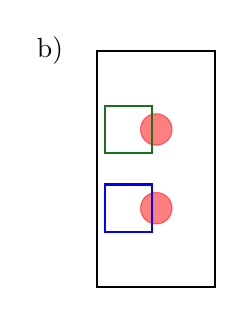
\begin{tikzpicture} 
      \node at (-0.6,3) {b)};
      \draw[thick] (0,0) rectangle (1.5,3);
      \draw[red,opacity=0.5, fill] (0.75,2) circle (0.2);   % pattern1
      \draw[red,opacity=0.5, fill] (0.75,1) circle (0.2);   % pattern1

      % readout windows
      \draw[thick,darkgreen] (0.1,1.7) rectangle (0.7,2.3);
      \draw[thick,blue] (0.1,0.7) rectangle (0.7,1.3);
    \end{tikzpicture} 
  };

  % Box 3: Stare
  \node[at={($(scope2.east)+(.6cm,0)$)},anchor=west](scope3){
    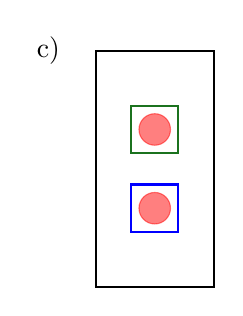
\begin{tikzpicture} 
      \node at (-0.6,3) {c)};
      \draw[thick] (0,0) rectangle (1.5,3);
      \draw[red,opacity=0.5, fill] (0.75,2) circle (0.2);   % pattern1
      \draw[red,opacity=0.5, fill] (0.75,1) circle (0.2);   % pattern1

      % readout windows
      \draw[thick,darkgreen] (0.45,1.7) rectangle (1.05,2.3);
      \draw[thick,blue] (0.45,0.7) rectangle (1.05,1.3);

    \end{tikzpicture} 
  };

  % Box 4: Move again
  \node[at={($(scope3.east)+(.6cm,0)$)},anchor=west](scope4){
    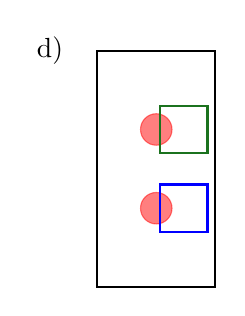
\begin{tikzpicture} 
      \node at (-0.6,3) {d)};
      \draw[thick] (0,0) rectangle (1.5,3);
      \draw[red,opacity=0.5, fill] (0.75,2) circle (0.2);   % pattern1
      \draw[red,opacity=0.5, fill] (0.75,1) circle (0.2);   % pattern1

      % readout windows
      \draw[thick,darkgreen] (0.8,1.7) rectangle (1.4,2.3);
      \draw[thick,blue] (0.8,0.7) rectangle (1.4,1.3);

    \end{tikzpicture} 
  };

  % Box 5: Readout 
  \node[at={($(scope4.east)+(.6cm,0)$)},anchor=west](scope5){
    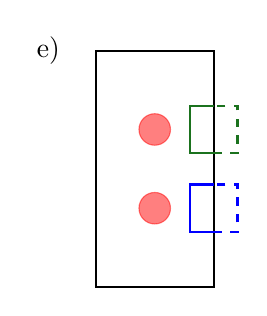
\begin{tikzpicture} 
      \node at (-0.6,3) {e)};
      \draw[thick] (0,0) rectangle (1.5,3);
      \draw[red,opacity=0.5, fill] (0.75,2) circle (0.2);   % pattern1
      \draw[red,opacity=0.5, fill] (0.75,1) circle (0.2);   % pattern1

      % readout windows
      \draw[thick,darkgreen,dashed] (1.5,1.7) -- (1.8,1.7) -- (1.8,2.3) -- (1.5,2.3);
      \draw[thick,darkgreen] (1.5,1.7) -- (1.2,1.7) -- (1.2,2.3) -- (1.5,2.3);

      \draw[thick,blue,dashed] (1.5,0.7) -- (1.8,0.7) -- (1.8,1.3) -- (1.5,1.3);
      \draw[thick,blue] (1.5,0.7) -- (1.2,0.7) -- (1.2,1.3) -- (1.5,1.3);

    \end{tikzpicture} 
  };

\end{tikzpicture}


\end{document}
